\subsection{Langkah Praktikum: Selection Sort D\&C}

\subsubsection*{Flowchart}
\begin{figure}[H]
    \centering
    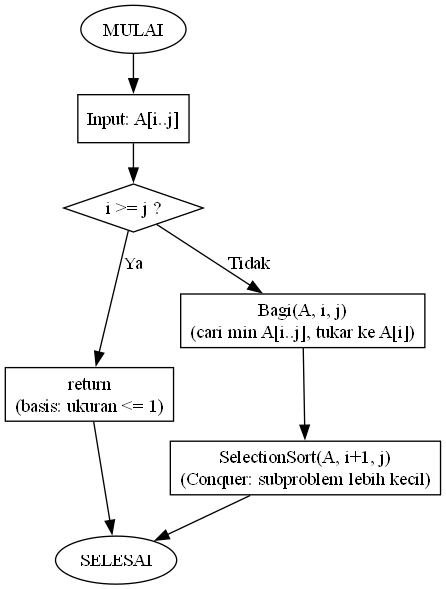
\includegraphics[width=0.45\textwidth]{figures/praktikum5/flowchart_selection_sort_dc.png}
    \caption{Flowchart Algoritma Selection Sort Decrease and Conquer}
\end{figure}

\subsubsection*{Source Code Python}
\begin{lstlisting}[basicstyle=\ttfamily\scriptsize, frame=single, backgroundcolor=\color{white}, numbers=none, keywordstyle=\color{black}, commentstyle=\color{black}, stringstyle=\color{black}, breaklines=true]
def bagi(arr, i, j):
    # cari indeks elemen terkecil dari A[i..j]
    idx_min = i
    for k in range(i + 1, j + 1):
        if arr[k] < arr[idx_min]:
            idx_min = k
            
    # tukar elemen terkecil ke posisi i
    arr[i], arr[idx_min] = arr[idx_min], arr[i]

def selection_sort_dc(arr, i, j):
    # basis: ukuran subarray <= 1, sudah terurut
    if i >= j:
        return
        
    # decrease: letakkan elemen terkecil A[i..j] ke posisi i
    bagi(arr, i, j)
    
    # conquer: urutkan sisa subarray A[i+1..j] secara rekursif
    selection_sort_dc(arr, i + 1, j)

if __name__ == "__main__":
    arr = [64, 25, 12, 22, 11]
    print("Data awal   :", arr)
    
    selection_sort_dc(arr, 0, len(arr) - 1)
    
    print("Data terurut:", arr)
\end{lstlisting}

\subsubsection*{Analisis Output}
Program dijalankan dengan data awal [64, 25, 12, 22, 11] sesuai modul:

\begin{table}[H]
    \centering
    \caption{Trace Rekursi Selection Sort D\&C}
    \begin{tabular}{lllll}
    \toprule
    \textbf{Rekursi ke} & \textbf{Subarray A[i..j]} & \textbf{Elemen Min} & \textbf{Setelah Bagi} & \textbf{Subproblem} \\ \midrule
    1 & A[0..4] = [64,25,12,22,11] & 11 (idx 4) & [11,25,12,22,64] & A[1..4] \\
    2 & A[1..4] = [25,12,22,64] & 12 (idx 2) & [11,12,25,22,64] & A[2..4] \\
    3 & A[2..4] = [25,22,64] & 22 (idx 3) & [11,12,22,25,64] & A[3..4] \\
    4 & A[3..4] = [25,64] & 25 (idx 3) & [11,12,22,25,64] & A[4..4] \\
    5 & A[4..4] = [64] & basis i>=j & tidak ada tukar & selesai \\ \bottomrule
    \end{tabular}
\end{table}

Output akhir: [11, 12, 22, 25, 64]. Setiap rekursi mereduksi submasalah sebesar 1 elemen (decrease by constant = 1). Tidak ada tahap combine karena posisi A[i] sudah final setelah setiap pemanggilan Bagi.

\subsection{Post Test: Selection Sort dengan Input Pengguna}

\subsubsection*{Source Code Python}
\begin{lstlisting}[basicstyle=\ttfamily\scriptsize, frame=single, backgroundcolor=\color{white}, numbers=none, keywordstyle=\color{black}, commentstyle=\color{black}, stringstyle=\color{black}, breaklines=true]
def bagi(arr, i, j):
    # cari indeks elemen terkecil dari A[i..j]
    idx_min = i
    for k in range(i + 1, j + 1):
        if arr[k] < arr[idx_min]:
            idx_min = k
            
    # tukar elemen terkecil ke posisi i
    arr[i], arr[idx_min] = arr[idx_min], arr[i]

def selection_sort_dc(arr, i, j):
    # basis: ukuran subarray <= 1, sudah terurut
    if i >= j:
        return
        
    # decrease: letakkan elemen terkecil ke posisi i
    bagi(arr, i, j)
    
    # conquer: rekursif pada subarray yang lebih kecil
    selection_sort_dc(arr, i + 1, j)

if __name__ == "__main__":
    # terima input array dari pengguna
    raw = input("Masukkan bilangan dipisah spasi: ")
    arr = list(map(int, raw.split()))
    
    print("Data awal   :", arr)
    selection_sort_dc(arr, 0, len(arr) - 1)
    print("Data terurut:", arr)
\end{lstlisting}

\subsubsection*{Analisis Output}
Program menerima input dari pengguna berupa bilangan yang dipisah spasi, mengonversinya ke list integer, lalu menjalankan Selection Sort D\&C. Contoh eksekusi dengan input "5 3 8 1 9 2":

\begin{table}[H]
    \centering
    \caption{Output Hasil Selection Sort Input Pengguna}
    \begin{tabular}{lll}
    \toprule
    \textbf{Input} & \textbf{Data Awal} & \textbf{Data Terurut} \\ \midrule
    5 3 8 1 9 2 & [5, 3, 8, 1, 9, 2] & [1, 2, 3, 5, 8, 9] \\ \bottomrule
    \end{tabular}
\end{table}

Implementasi ini membuktikan bahwa Selection Sort berbasis Decrease and Conquer menghasilkan output yang identik dengan versi iteratif, dengan alur rekursi yang lebih eksplisit mencerminkan prinsip decrease by a constant.